\section*{ 3 Examen des données, prétraitements et extraction des de
scripteurs}

\subsection*{Question 3.1: Compléter la fonction
preprocessing() permettant de charger les deux images et de
les afficher. indication:
loadImages() .} 
\label{code1}


\begin{lstlisting}[caption={Fonction de prétraitement}, label={code1}] 
import numpy as np
import matplotlib.pyplot as plt

from loadImages import loadImages
from selectFeatureVectors import selectFeatureVectors
from displayFeatures2d import displayFeatures2d
from displayFeatures3d import displayFeatures3d


#%% def preprocessing
def preprocessing():

    img73, img87 = loadImages()

    fig = plt.figure(figsize=(10,6))
    plt.subplot(121)
    plt.imshow(img73)
    plt.title("Aral Sea - 1973")

    plt.subplot(122)
    plt.imshow(img87)
    plt.title("Aral Sea - 1987")

    plt.show()

    featLearn, nbPix, nbFeat = selectFeatureVectors(img73, 10)
   
    return featLearn,img73,img87

if __name__ == "__main__":
    preprocessing()


\end{lstlisting}

\begin{figure}[H]
    \centering
    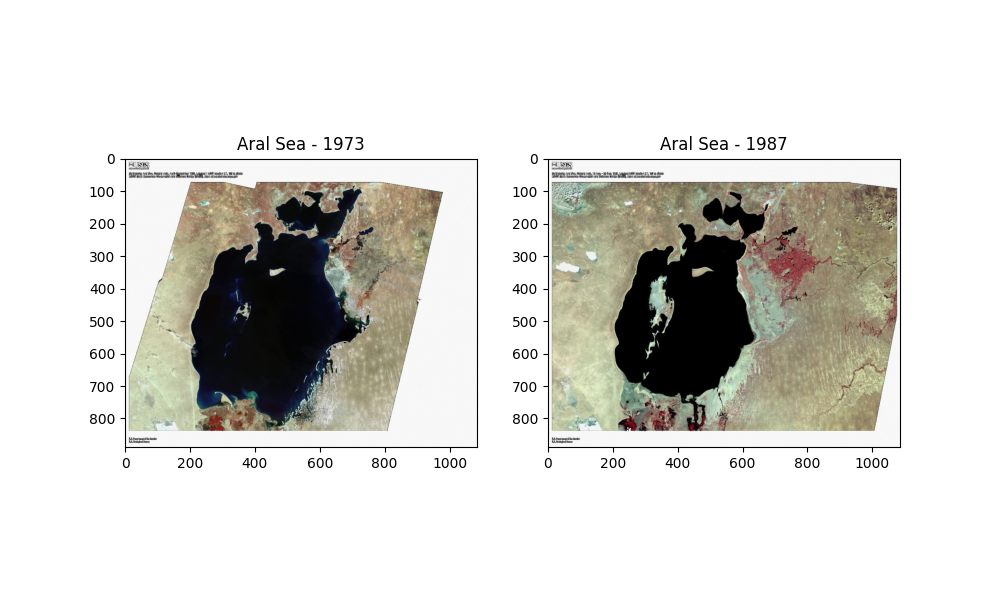
\includegraphics[width=1\linewidth]{figure/Figure_1.png}
    \label{fig:placeholder}
\end{figure}


\subsection*{Question 3.2: Que peut-on déduire de l'analyse de ces images ? Comment sont codées les valeurs des pixels ?}

\begin{itemize}
    \item L'analyse de ces images permetre de visualiser l'asséchement de la mer d'Aral. On observe une diminution de la surface d'eau bleue.
    Les images chargées sont de matrices 3D où chaque pixel est codé sur 3 canaux, ils sont rouge, vert et blueu. 
\end{itemize}

\subsection*{Question 3.3: Les images sont en couleurs et nous allons utiliser les composantes des couleurs comme
descripteurs de classification. Quelle est la dimension de l’espace des descripteurs lorsque l’image
est codée en RGB (RVB) ?}
\begin{itemize}
    \item La dimension de l'espace des descripteurs est de 3. Chaque pixel est répresenté par un vecteur contenant trois valeurs : vec\_pix = [rouge, vert, bleu].
\end{itemize}

\subsection*{Question 3.4: Tronquer de la même manière les deux images pour faire disparaître le texte dans la
partie haute et basse des images.}

Pour tronquer les deux images il suffit d'ajouter ces deux lignes de codes dans \ref{code1} :

\begin{lstlisting}
    margin = 50 
    im73 = im73[margin+10:-margin, :, :]
    im87 = im87[margin+10:-margin, :, :]
\end{lstlisting}

\section*{4 Constitution d’un ensemble de données d’apprentissage}
\subsection*{Question 4.1: Compléter la fonction
preprocessing() par une partie qui vise à constituer une base
d’apprentissage. Pour cela, réalisez un sous-échantillonnage de l’image de 1973 avec un pas de 500
points (indication :
selectFeatureVectors.py ). Quel est le nombre de données d’apprentissage?}

On peut ajouter ces lignes de code :

\begin{lstlisting}
    ...
    featLearn, nbPix, nbFeat = selectFeatureVectors(img73, 500)

    print("Nombre de donnees dapprentissage : ", nbPix)
    
\end{lstlisting}

Comme sortie on a :

\begin{figure}[H]

    \centering
    \includegraphics*[width=1\linewidth]{figure/sortie.png}
    
\end{figure}

\section*{5 Première analyse des données}

\subsection*{Question 5.1: Dans
preprocessing.py , visualiser en 2D et 3D les valeurs des descripteurs. La visu
alisation en 2D des vecteurs d’apprentissage se fait par la fonction
displayFeatures2d(feat) et
en 3D
displayFeatures3d(feat) .}

\begin{figure}[H]

    \centering
    \includegraphics*[width=1\linewidth]{figure/Figure_2D.png}
    
\end{figure}

\begin{figure}[H]

    \centering
    \includegraphics*[width=1\linewidth]{figure/Figure_3D.png}
    
\end{figure}

\subsection*{Question 5.2: Décrivez explicitement ces graphiques en expliquant ce qu’ils représentent, en donnant
leurs caractéristiques pour les histogrammes et les nuages de points (différents groupes? à quelles
informations peut-on les relier?)}

\begin{itemize}
    \item Les histogrammes sur la diagonale principale montrent qu'il y a plein des pixels avec des valeurs proches de 0-20 d'intensité
    et 150-250 d'intensité, dans ce façon est possible affirmer que ces valeus plus basses sont liées à l'eau et les valeurs plus haute
    ont un fort liason avec terre/sable. Les nuages hors diagonale montrent une forte correlation linéaire entre les trois canaux. L'image 
    3D affichent qu'on a une certaine dvision de deux groupes de pixels, les pixels avec des valeurs plus basses et les pixels avec valeurs
    plus haut, comme ça est possible de diviser les pixels en deux groupes.
\end{itemize}